\subsubsection{Financials Use Case}
\paragraph{Scenario 1: Check only}
\subparagraph{Generic Steps - Event Based:}
\begin{itemize}
\item Client sends request to Client-Side Middleware to verify specific data (data or indexes are not known by Client)
\item Client-Side Middleware triggers relevant Smart Contract function
\item Smart Contract triggers Event to retrieve specific data
\item Client-Side Middleware listens to Event and queries required data from the database
\item Client-Side Middleware sends required data to smart contract via function call
\item Smart Contract checks integrity
\item Smart Contract triggers Event to send result of integrity check (result = corrupted records or true/false)
\item Client-Side Middleware listens to Event and sends the result back to client
\end{itemize}

\subparagraph{Generic Steps - Data to check is Known:}
\begin{itemize}
\item Client sends request to Client-Side Middleware to verify specific data (data or indexes are not known by Client)
\item Client-Side Middleware queries required data from the database
\item Client-Side Middleware sends required data to smart contract via function call
\item Smart Contract checks integrity
\item Smart Contract triggers Event to send result of integrity check (result = corrupted records or true/false)
\item Client-Side Middleware listens to Event and sends the result back to client
\end{itemize}

\paragraph{Concept - Financials}
\subparagraph{Description}
An external auditor wants to check the financial situation of a company. One task could be to check the stated weekly or monthly sales amount against the sum of all sales records in the specific year. One of the first steps would be to verify (check the integrity) of all sales records in the specific year.

This use case consists of two parties, a financial auditor and the company that holds the financial data. An assumption that we make is that the middleware is open-sourced, produced by an auditing company, and it is being consumed by the company to store their financial data in the Blockchain environment. The middleware allows the company to off-chain their financial records from the Smart Contract into a database, while maintaining the integrity of the data using the Blockchain environment. The middleware also allows the auditor to easily audit companies’ financial records without having to worry about the integrity of data once they are appended. It also allows the auditor to query the financial records with a filter, such as the date of the records, performing query completeness. The middleware however does not allow users to edit the records through the middleware, though it is possible to do it on the database directly, which will then result in an integrity check error when the records are used or verified by the auditor. 

\textit{Example: A Sales Table}
\begin{center}
    \begin{tabular}{| l | l | l | l | l |}
    \hline
    ID & Product & Date & Amount & Price \\ \hline
    1 & Wallet & 20171230 & 1 & 20 \\ \hline
    .. & ... & .... & .. & ... \\ \hline
    \end{tabular}
\end{center}

The different table rows represent moments in time (e.g. every Friday night after 00:00 or every first of the month) and thus new records are appended to the table. In this way, the records can be tracked back in time and an auditor could double-check the records for e.g. the last 6 months or the last 104 weeks. The Smart Contract entry then consists of the root hash over every table row (with each column being a leaf in the Merkle tree).

As the database is under the control of the company storing their financial figures, the financial auditor cannot be sure that those numbers were inserted correctly (same as without blockchain). By having the hashes of the records on the blockchain, the auditor can be sure that the company was not able to change the figures later on and thus has the certainty that there are no accounting tricks and malpractices in place e.g. at the end of the year or quarter. The figures that were once recorded by the company can be double-checked afterwards (or it can be noticed that the company recorded wrong numbers or tried to change them in hindsight). It is worth mentioning that the Smart Contract never stores the financial figures and they are thus not available on the blockchain either. While upon insertion, there isn’t a way to check that the numbers are true, but we can assert that these numbers will not be prone to illegitimate changes. 

Furthermore, this use case could be valuable for rewarding benefits to employees. For example, the CEO of a company could receive a benefit by the shareholders (indirectly through the company itself but signed by the shareholders) if certain financial data are met. Or a sales person in the company could receive a benefit for sales data records for a certain month that went especially well. 

To conclude, this use case asserts that large quantities of data (like financial figures of a company) cannot be modified after reporting them while only storing a relatively cheap representation of that data (hash) on the blockchain. Third parties and internal controllers are thus able to rely on the integrity of the recorded data. 

\paragraph{Implementation - Financials}
\subparagraph{Initial Concept: Whole Table Verification}

In this initial approach and concept, we created an assumption that the financial rows are prone to changes, and that the Smart Contract is going to keep track of the total or the aggregation of the rows. Hence, a verification of the whole table is needed to ultimately maintain the integrity of the “Total” row.

The Smart Contract stores the current root hash of the whole table. It could also store the root hashes of the prior states of the table (this info could otherwise be found in the blockchain history) to allow for additional functionalities.

The Smart Contract creates a Merkle tree over the hashes of all rows. The hashes of the rows are provided by the middleware. Afterwards, the Smart Contract verifies that the root hash of the created Merkle tree matches the stored current root hash. If that is the case, it calculates the new total value(s), and adds the hash of the new row (new entry) to the Tree to create the new root hash after these processes. This new root hash is then stored as the current one. 

Merkle tree is used here when a column, or multiple column values are changed in a row, and we need to recalculate the new values for the Total row. Instead of verifying the whole data in a row, we only need to verify the nodes that are affected by the change. 

For the Merkle tree implementation, there is no need to implement a new one or change the existing one, as we can use the Multiple Item Proof here (note: an item here will correspond to a row, not a column).

Append row - Steps:
\begin{enumerate}
\item First, the client side application gets all the data from the Database.
\item It then creates the proof and sends it to the Smart Contract.
\item The Smart Contract does the integrity check. 
\item Now, first the new total values are calculated, the Smart Contract 
\item creates a root hash for that total row, then recreates the tree with 
\item that new roothash from the total row, and that newly added item row. 
\item Send back the total row, and that newly added item row. 
\end{enumerate}

\subparagraph{Realization}

We quickly realized the “red flags” this approach is producing in regards to the gas cost. In the process of adding a new row, we are adding a new leaf, or a new hash into the current Merkle tree (step 4), and this does not work that way, as we are planning on having only the Merkle proof, the nodes that are not affected by the change. Hence, to approach this we always have to send all of the leaves, the hashes of the rows, so that we can create this new tree in addition to a new leaf, the new hash of the inserted row. This quickly creates an overhead in the gas cost when adding a new row into the table. Hence, we took a turn in our approach, and we have to come up with something more usable, and worth it for the users. While the same gas cost problem will still exist in the next approach, it will however provide a much larger incentive for using the function. 

\subparagraph{Query Completeness}

Query completeness is the concept that we came up with that can better leverage the whole table verification. Furthermore, it addresses an important real-world problem. A user queries the database, however, does not want to put trust into the returned results. The blockchain can be used as an objective verifier of the query results. See section \ref{sssec: queryCompleteness} to learn more about the concept. An example on how this mechanism is applied to our use case includes a user who wants to query all sales data in the period from Nov 2017 to Jan 2018, and expects that the results have not been tampered with. 


Initial implementation idea:
\begin{itemize}
\item Verify that all entries were considered and that none were left out in the returned results.
→  have database respond to original query and to the negated query (e.g. original: all sales data in the period from Nov 2017 to Jan 2018, negated: all sales data NOT in the period from Nov 2017 to Jan 2018)
→ check that combined size of both returned lists equals total number of entries (mapping counter in SC)
\item Verify that only actual entries from the database were returned
→ combine the two result lists to one Merkle proof to show that all rows are part of the table, i.e. no entries were changed and no outside entries were returned as a result
\item Verify that the returned results match the query requirements (are “correct”)
→ no feasible way with blockchain currently as we would either need to do a lot of computation or to store a large amount of data (maybe even all data) on-chain, which would contradict this project’s focus
→ leave this verification up to the user (she can see whether the results match her query)
\item Verify that all results that match the query were actually returned
→ no feasible way with blockchain currently as we would either need to do a lot of computation or to store a large amount of data (possibly even all data) on-chain, which would contradict this project’s focus
→ unfortunately, the user does not have an easy way to verify that either
\end{itemize}

The above statements show that there is a clear trade-off between achieving Query Completeness and this project’s goal of saving gas costs by off-chaining data. Either practically all data has to be stored on-chain to enable our smart contract to guarantee Query Completeness, or a plethora of computations (Merkle proofs for each row in the data table) have to be on-chained which would hit the gas limit relatively fast. 

As we are facing the challenge described previously, we decided to implement our proof of concept for Query Completeness by adding assumptions to make it feasible and easier for testing for large amount of data: building on our initial assumption that we trust our client-side application, we calculate the Merkle proofs on the client-side and thus save a considerable amount of computation on-chain. Nevertheless, the smart contract will check the integrity of the data and perform a simplified query to guarantee Query Completeness. We also only allow the Date column to be used in the query in this proof of concept

\subparagraph{Proof of Concept}

This section describes the step-by-step actions between our client-side application, Smart Contract and the Database. The proof of concept includes the implementation of appending a new financial row, and query completeness. We want to remind the readers to keep in mind the previous assumptions that we have stated. 


\textit{Example: This table shows how the records are stored in the database, assuming all data here are appended through the Smart Contract.}
\begin{center}
    \begin{tabular}{| l | l | l | l | l | l | l | l |}
    \hline
    ID & company\_name & roothash & total\_sales & date & cogs & sc\_id & ... \\ \hline
    1 & CompanyAB & 0x123 & 1000 & 20160523 & 123 & 0 & .. \\ \hline
    2 & CompanyAB & 0x134 & 2000 & 20161215 & 421 & 1 & .. \\ \hline
    3 & CompanyAB & 0x321 & 3000 & 20170601 & 222 & 2 & .. \\ \hline
    4 & CompanyAB & 0x789 & 9000 & 20180130 & 980 & 3 & .. \\ \hline
    \end{tabular}
\end{center}



\textbf{\textit{Appending A Finanical Row}}

\begin{figure}[h]%evtl:[t] [!htbp]
\centering
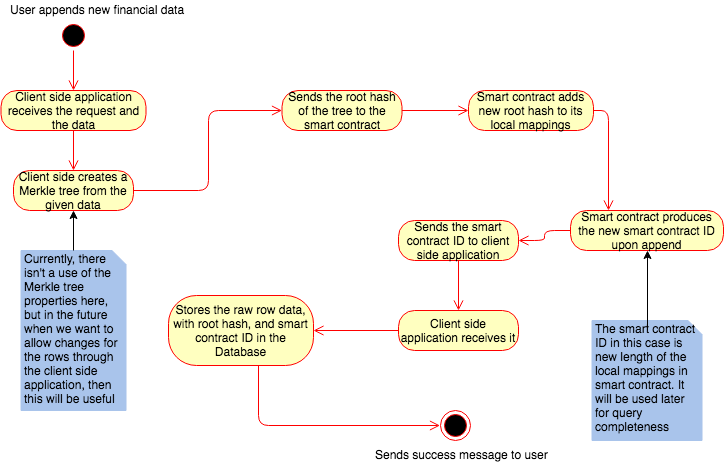
\includegraphics[width=1.0\textwidth]{images/appendRowFinancials.png}
\caption{\label{fig:appendRowFinancials}Activity diagram of appending a row to the financials record}
\end{figure}

\begin{enumerate}
\item User appends a new financial data, providing all the required information to be in the database
\item Client-side application then creates a Merkle tree from the given raw data
\item Sends the root hash of the created Merkle tree to the Smart Contract 
\item Smart Contract appends that new root hash into its local mappings. 
\item Smart Contract increments the new length of the mapping, which is the Smart Contract ID that is going to be returned. This acts as an identifier to which hash belongs to which financial row. It is also used to preserve the ordering of the hashes which will later be used for Query Completeness. 
\item Smart Contract sends back the Smart Contract ID to the client-side application
\item Client-side application saves the raw financial data, with the root hash, and the Smart Contract ID. 
\end{enumerate}

\textbf{\textit{Query Completeness}}

\begin{figure}[h]%evtl:[t] [!htbp]
\centering
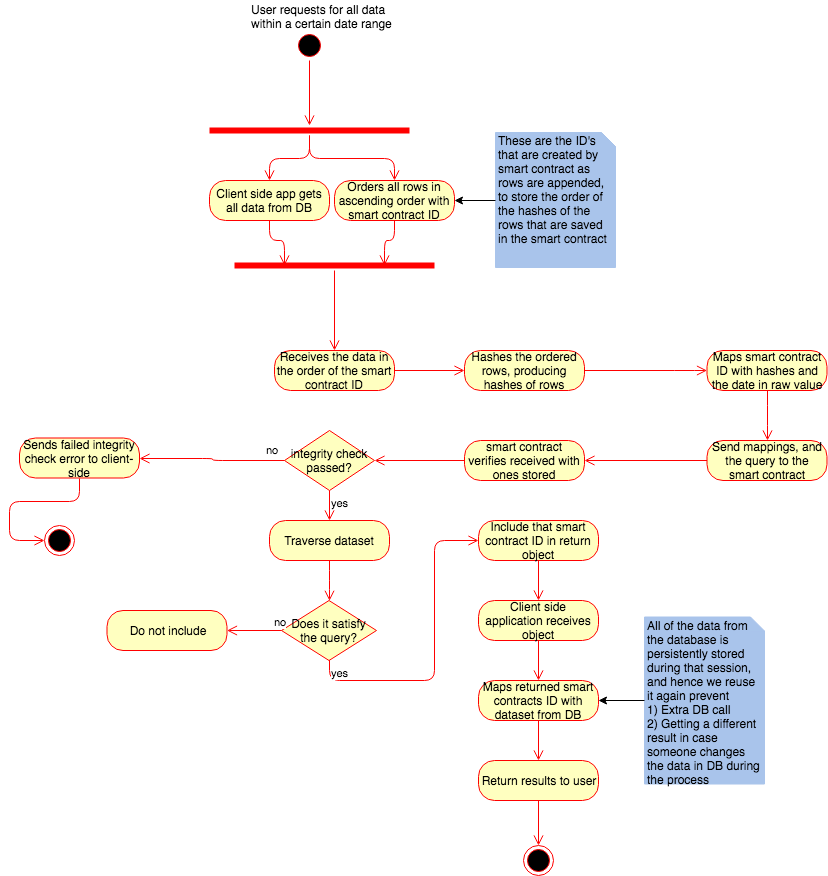
\includegraphics[width=1.0\textwidth]{images/queryCompleteness.png}
\caption{\label{fig:queryCompleteness}Activity diagram for query completeness}
\end{figure}


\begin{enumerate}
\item User requests to get all of financial data that are within the data range the user has requested.
\item The client-side application gets all data from the database in the ascending order of the Smart Contract ID. This ID is generated by the Smart Contract to keep the ordering of the hashes that are stored in the Smart Contract. It is generated upon appending a financial record through the Smart Contract. 
\item The client-side application hashes all the returned rows
\item It will then maps the hashes of the row and the raw date value to the Smart Contract ID.  
\item The client-side application sends the mapping with the query to the Smart Contract.
\item The smart contract checks if it got the right data, the right amount of rows and the correct table overall by iterating over the provided root hashes and comparing them to the previously stored ones.
	\begin{enumerate}
	\item If Smart Contract cannot verify the rows, then it will throw an integrity check error to the client-side application as an event. 
	\item If the smart contract can confirm this, it checks the query condition for every row and returns (better: puts into an event) an array of booleans indicating all the indexes of rows that fulfill the query. Dates are intentionally stored as “uint” to ease the query function in the smart contract. For example 1, March, 2018 -> 20180301
	\end{enumerate}
\item Smart Contract returns back all the Smart Contract IDs that have satisfied the query.
\item The client-side application listens to this event and returns the specified rows to the user subsequently.
\end{enumerate}



